% CampusWatch project guide. Build:  tectonic docs/CampusWatch_Project_Guide.tex
\documentclass[11pt,a4paper]{article}

\usepackage{fontspec}
\setmainfont{texgyrepagella}[Extension=.otf, UprightFont=*-regular, BoldFont=*-bold, ItalicFont=*-italic, BoldItalicFont=*-bolditalic]
\setsansfont{texgyreheros}[Extension=.otf, UprightFont=*-regular, BoldFont=*-bold, ItalicFont=*-italic, BoldItalicFont=*-bolditalic]
\setmonofont{lmmono10-regular.otf}

\usepackage[margin=2.3cm, headheight=14pt]{geometry}
\usepackage{xcolor}
\usepackage{tikz}
\usetikzlibrary{positioning, arrows.meta, fit, backgrounds, calc}
\usepackage[most]{tcolorbox}
\usepackage{booktabs, tabularx, longtable, array}
\usepackage{listings}
\usepackage{enumitem}
\usepackage{titlesec}
\usepackage{fancyhdr}
\usepackage{amsmath, amssymb}
\usepackage{needspace}
\usepackage[hidelinks]{hyperref}

\definecolor{ink}{HTML}{1B2430}
\definecolor{muted}{HTML}{5B6676}
\definecolor{accent}{HTML}{1F9FBC}
\definecolor{rule}{HTML}{D5DBE3}
\definecolor{codebg}{HTML}{F4F6F9}
\definecolor{acad}{HTML}{3987E5}
\definecolor{admin}{HTML}{D95926}
\definecolor{stu}{HTML}{199E70}
\definecolor{dc}{HTML}{9085E9}
\definecolor{okc}{HTML}{1E9E5A}
\definecolor{warnc}{HTML}{C98500}
\definecolor{critc}{HTML}{D64545}

\hypersetup{colorlinks=true, linkcolor=accent, urlcolor=accent}
\setlength{\parindent}{0pt}
\setlength{\emergencystretch}{3em}
\setlength{\parskip}{6pt}
\renewcommand{\arraystretch}{1.25}
\setlist{itemsep=2pt, topsep=4pt}

\titleformat{\section}{\sffamily\Large\bfseries\color{ink}}{\thesection}{0.8em}{}[\vspace{-2pt}{\color{rule}\titlerule}]
\titleformat{\subsection}{\sffamily\large\bfseries\color{ink}}{\thesubsection}{0.7em}{}
\titleformat{\subsubsection}{\sffamily\normalsize\bfseries\color{ink}}{}{0em}{}
\titlespacing*{\section}{0pt}{18pt}{8pt}

\pagestyle{fancy}
\fancyhf{}
\fancyhead[L]{\sffamily\small\color{muted}CampusWatch: Smart Campus Network Monitor}
\fancyhead[R]{\sffamily\small\color{muted}Project guide}
\fancyfoot[C]{\sffamily\small\color{muted}\thepage}
\renewcommand{\headrulewidth}{0.4pt}
\renewcommand{\headrule}{\color{rule}\hrule width\headwidth height\headrulewidth}

\lstdefinestyle{shell}{basicstyle=\ttfamily\small, backgroundcolor=\color{codebg}, frame=single, rulecolor=\color{rule},
  framesep=6pt, xleftmargin=6pt, xrightmargin=6pt, columns=fullflexible, keepspaces=true, breaklines=true,
  showstringspaces=false, aboveskip=6pt, belowskip=6pt}
\lstset{style=shell}

\newtcolorbox{keyidea}[1][Key idea]{colback=accent!6, colframe=accent, boxrule=0.6pt, arc=2pt, left=8pt, right=8pt,
  top=4pt, bottom=4pt, fonttitle=\sffamily\bfseries\small, coltitle=white, title=#1}
\newtcolorbox{sayit}{colback=okc!6, colframe=okc, boxrule=0.6pt, arc=2pt, left=8pt, right=8pt, top=4pt, bottom=4pt,
  fonttitle=\sffamily\bfseries\small, coltitle=white, title=How to say it}
\newtcolorbox{careful}{colback=warnc!7, colframe=warnc, boxrule=0.6pt, arc=2pt, left=8pt, right=8pt, top=4pt, bottom=4pt,
  fonttitle=\sffamily\bfseries\small, coltitle=white, title=Be careful}

\newcommand{\code}[1]{\texttt{#1}}
\newcommand{\file}[1]{\texttt{\color{ink}#1}}
\newcommand{\qa}[2]{\par\textbf{\sffamily Q. #1}\par\vspace{-2pt}#2\par\vspace{4pt}}

\newcolumntype{Y}{>{\raggedright\arraybackslash}X}
\let\oldsection\section\renewcommand{\section}{\needspace{12\baselineskip}\oldsection}
\let\oldsubsection\subsection\renewcommand{\subsection}{\needspace{8\baselineskip}\oldsubsection}
\begin{document}

% ------------------------------------------------------------------ title
\begin{titlepage}
\vspace*{3cm}
{\sffamily\color{accent}\large Computer Networks project\par}
\vspace{6pt}
{\sffamily\bfseries\fontsize{34}{38}\selectfont\color{ink} CampusWatch\par}
\vspace{4pt}
{\sffamily\Large\color{ink} Smart Campus Network Monitor\par}
\vspace{18pt}
{\large\color{muted} Project guide: what it is, how it works, how to run it,\\ how to demonstrate it and how to explain it.\par}
\vspace{2cm}
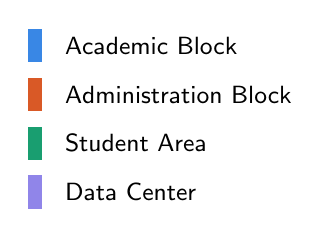
\begin{tikzpicture}
  \foreach \c/\n [count=\i] in {acad/Academic Block, admin/Administration Block, stu/Student Area, dc/Data Center} {
    \fill[\c] (0,-\i*0.62) rectangle ++(0.18,0.42);
    \node[anchor=west, font=\sffamily\small] at (0.35,-\i*0.62+0.21) {\n};
  }
\end{tikzpicture}
\vfill
{\sffamily\small\color{muted}
Backend: Python 3.11+ with FastAPI, SQLAlchemy, SQLite, psutil, pysnmp and scikit-learn.\\
Frontend: React and TypeScript with Vite, Tailwind CSS and Recharts.\\[4pt]
Companion documents in the repository:\\
\file{README.md} $\cdot$ \file{project.md} $\cdot$ \file{docs/architecture.md}\\
\file{docs/demo-guide.md} $\cdot$ \file{docs/Packet\_Tracer\_Topology.pdf}\par}
\end{titlepage}

\tableofcontents
\newpage

% ------------------------------------------------------------------ 1
\section{How to use this guide}

This guide is for whoever presents CampusWatch. Read it in this order:

\begin{enumerate}
  \item \textbf{Sections 2 and 3} (15 minutes): what the project does and the networking ideas behind it.
  \item \textbf{Section 5} (20 minutes): install and run it on your laptop. Do this at least a day before the presentation.
  \item \textbf{Section 7} (15 minutes): rehearse the demo script twice with the app open.
  \item \textbf{Section 8} (30 minutes): the questions a professor is likely to ask, with answers. Say the answers in your own words.
  \item \textbf{Sections 4, 9 and 10} when you need detail: architecture, where the code for each feature lives, limitations.
\end{enumerate}

Green \emph{How to say it} boxes give short explanations you can use out loud. Orange \emph{Be careful} boxes mark the places where
a precise answer matters, usually about what is real data and what is simulated.

% ------------------------------------------------------------------ 2
\section{The project in one page}

\textbf{Problem.} A campus network has several buildings (areas), each on its own VLAN and subnet, connected through switches and
a core router. An administrator wants to know, at a glance: which devices are up, how much traffic each area and link carries,
which links are close to full (congestion), and when traffic does something unusual (anomalies). They also want history,
to compare areas and see trends.

\textbf{What CampusWatch does.}
\begin{itemize}
  \item \textbf{Collects} interface byte counters and device status every 10 seconds (configurable).
  \item \textbf{Computes} traffic rates (bits per second) from the difference between two counter readings, and link utilization
        when the link capacity is known.
  \item \textbf{Stores} every sample in a SQLite database for history (7 days by default).
  \item \textbf{Detects} congestion (utilization thresholds), traffic spikes (rolling statistical baseline), optional machine-learning
        anomalies (Isolation Forest), unreachable devices and collector errors, and turns them into deduplicated alerts.
  \item \textbf{Shows} everything in a custom web dashboard: overview, devices and interfaces, traffic analytics, alerts, settings.
\end{itemize}

\textbf{Three collection modes} (switchable in Settings, no code changes):
\begin{center}
\begin{tabularx}{\linewidth}{@{}l Y Y@{}}
\toprule
\textbf{Mode} & \textbf{Data source} & \textbf{When to use} \\
\midrule
Demo  & A built-in generator that simulates a campus (4 areas, 15 devices, 17 interfaces) with daily patterns, congestion and spikes.
        Clearly labelled \emph{synthetic} everywhere. & Presentations; works with no network equipment. \\
Local & Real counters from the laptop's own network interfaces (Python \code{psutil}). & Showing real, live measurement. \\
SNMP  & Real routers and switches polled over SNMP v2c or v3 (IF-MIB counters). & A lab with reachable SNMP-enabled devices. \\
\bottomrule
\end{tabularx}
\end{center}

\begin{keyidea}[The principle that runs through the whole project]
Never show a number that was not measured. Demo data is always labelled synthetic. A rate is only shown after two readings.
Utilization is only shown when the link capacity is known. An unreachable device shows ``n/a'', never zero. SNMP failures are
shown with the exact error, never hidden.
\end{keyidea}

% ------------------------------------------------------------------ 3
\section{Networking concepts you must be able to explain}

\subsection{Interface counters and why a rate needs two readings}

Every network interface keeps two \emph{cumulative} counters: total bytes received (\emph{in}) and total bytes sent (\emph{out})
since it started. A single counter value (for example 8\,214\,553\,190 bytes) says nothing about the current speed. To get a
rate you take two readings and divide the difference by the time between them:

\[
\text{rate}_{\text{bps}} \;=\; \frac{(\text{bytes}_{\text{now}} - \text{bytes}_{\text{before}}) \times 8}{t_{\text{now}} - t_{\text{before}}}
\]

The $\times 8$ converts bytes to bits, because link speeds are quoted in bits per second (Mbps, Gbps).

\textbf{Worked example.} At 10:00:00 the in-counter is 1\,000\,000 bytes; at 10:00:10 it is 13\,500\,000 bytes.
Difference: 12\,500\,000 bytes $= 100\,000\,000$ bits in 10\,s, so the inbound rate is 10\,000\,000\,bps $=$ \textbf{10\,Mbps}.

\textbf{Edge cases the code handles} (all in \file{backend/app/services/rates.py}):
\begin{itemize}
  \item \textbf{First poll:} there is no previous reading, so no rate. The sample stores the counter only.
  \item \textbf{Zero or negative elapsed time:} no rate (would divide by zero or go backwards).
  \item \textbf{32-bit counter wrap:} old SNMP counters (\code{ifInOctets}) are 32-bit and roll over at $2^{32}$ bytes
        (about 4.3\,GB). If the new value is smaller, the code adds $2^{32}$ once.
        Example: before $= 4\,294\,967\,000$, now $= 1\,704$ $\Rightarrow$ difference $= 1\,704 + 2^{32} - 4\,294\,967\,000 = 2\,000$ bytes.
  \item \textbf{Counter reset} (device rebooted): on 64-bit counters a smaller value means a reset, so that interval is skipped.
  \item \textbf{Impossible value:} a rate above 110\% of the known link capacity is discarded as a misread counter.
  \item \textbf{Missing data:} an offline device writes no sample at all, so charts show a gap, not a fake zero.
\end{itemize}

\begin{sayit}
``Counters only ever go up, so one reading tells you nothing about speed. We read them every 10 seconds, subtract, multiply by
eight to get bits, and divide by the time. If we only have one reading, or the counter reset, we show \emph{unavailable}
instead of guessing.''
\end{sayit}

\subsection{Link capacity and utilization}

Utilization is how full a link is, as a percentage of its capacity:
\[
\text{utilization} = \frac{\max(\text{in}_{\text{bps}},\ \text{out}_{\text{bps}})}{\text{capacity}_{\text{bps}}} \times 100\%
\]
Ethernet links are \emph{full duplex}: each direction has the full capacity on its own, so the busier direction decides how
full the link is. Example: 80\,Mbps in and 10\,Mbps out on a 100\,Mbps link is \textbf{80\%}.

Capacity comes from (1) a value the administrator types in (always wins), (2) the speed the device reports
(SNMP \code{ifHighSpeed}/\code{ifSpeed}, or psutil), or (3) a default set on the SNMP target. If none is known, CampusWatch shows
the rate but \textbf{no utilization}. Many Wi-Fi adapters report no speed, which is why Local mode often shows ``n/a''.

\subsection{SNMP in short}

\begin{itemize}
  \item \textbf{Roles:} the \emph{manager} (CampusWatch) asks; the \emph{agent} on each router or switch answers. Requests go to UDP port 161.
  \item \textbf{MIB and OID:} data is organised as a tree; each value has an Object Identifier (OID), for example
        \code{1.3.6.1.2.1.1.3.0} is \code{sysUpTime}.
  \item \textbf{Operations used:} \code{GET} (one value) and \code{GETBULK} walks (a whole table column, efficiently).
  \item \textbf{Versions:} v2c authenticates with a \emph{community string} sent in clear text (lab only, read-only).
        v3 adds a username, authentication (SHA) and encryption (AES). CampusWatch supports both and recommends v3.
\end{itemize}

OIDs CampusWatch polls (IF-MIB unless noted):
\begin{center}
\small
\begin{tabularx}{\linewidth}{@{}l l Y@{}}
\toprule
\textbf{Object} & \textbf{OID} & \textbf{Used for} \\
\midrule
sysDescr, sysUpTime & 1.3.6.1.2.1.1.1 / .1.3 & reachability check, device description \\
ifDescr / ifName & 1.3.6.1.2.1.2.2.1.2 / 1.3.6.1.2.1.31.1.1.1.1 & interface names \\
ifType & 1.3.6.1.2.1.2.2.1.3 & skip loopback interfaces \\
ifOperStatus & 1.3.6.1.2.1.2.2.1.8 & up / down \\
ifHCInOctets, ifHCOutOctets & 1.3.6.1.2.1.31.1.1.1.6 / .10 & 64-bit byte counters (preferred) \\
ifInOctets, ifOutOctets & 1.3.6.1.2.1.2.2.1.10 / .16 & 32-bit fallback counters \\
ifHighSpeed / ifSpeed & 1.3.6.1.2.1.31.1.1.1.15 / 1.3.6.1.2.1.2.2.1.5 & link capacity \\
hrProcessorLoad, hrStorage & 1.3.6.1.2.1.25.3.3.1.2, 1.3.6.1.2.1.25.2.3.1 & CPU and memory (HOST-RESOURCES-MIB, best effort) \\
\bottomrule
\end{tabularx}
\end{center}

\textbf{Why 64-bit counters matter:} a 32-bit byte counter on a busy 1\,Gbps link wraps every
$2^{32} \times 8 / 10^9 \approx 34$ seconds, so one missed poll would make the rate ambiguous. The 64-bit HC counters effectively
never wrap.

\subsection{VLANs, subnets and campus areas}

Each campus area is a separate broadcast domain (VLAN) with its own IP subnet:

\begin{center}
\begin{tabular}{@{}l c l l@{}}
\toprule
\textbf{Area} & \textbf{VLAN} & \textbf{Subnet} & \textbf{Gateway} \\
\midrule
{\color{acad}$\blacksquare$} Academic Block & 10 & 192.168.10.0/24 & 192.168.10.1 \\
{\color{admin}$\blacksquare$} Administration Block & 20 & 192.168.20.0/24 & 192.168.20.1 \\
{\color{stu}$\blacksquare$} Student Area & 30 & 192.168.30.0/24 & 192.168.30.1 \\
{\color{dc}$\blacksquare$} Data Center & 100 & 10.10.0.0/24 & 10.10.0.1 \\
\bottomrule
\end{tabular}
\end{center}

Traffic between areas has to be routed. In the Packet Tracer build (separate PDF) one router does this with
\emph{router-on-a-stick}: a single trunk link carrying all VLANs, with one sub-interface (and gateway address) per VLAN.
The colours above are the same colours the dashboard uses for each area.

\subsection{Congestion detection}

A link is \emph{congested} when its utilization stays above a threshold:
\begin{itemize}
  \item \textbf{Warning} at $\geq 70\%$, \textbf{critical} at $\geq 90\%$ (both configurable).
  \item It must stay above the threshold for \textbf{2 consecutive samples} (configurable), so one short burst does not alert.
  \item \textbf{One alert per link} (deduplication). While the problem lasts, the same alert is updated (its occurrence count goes up)
        and can escalate from warning to critical.
  \item When utilization falls below the warning level, the alert is \textbf{resolved} automatically.
  \item If the same problem returns within the \textbf{cooldown} (10 minutes), the old alert is re-opened instead of creating a new one.
        This prevents alert flooding on a link that hovers around the threshold.
\end{itemize}

\subsection{Anomaly detection (traffic spikes)}

\textbf{Rule-based detector (always on).} For each interface it keeps the last 30 samples of total traffic (in + out) as a
\emph{rolling baseline}. For each new sample:
\[
z = \frac{x - \mu}{\sigma}, \qquad \text{flag if } z \geq 3 \ \text{ and } \ x \geq 1.6\,\mu \ \text{ and } \ x \geq 1\text{ Mbps}
\]
where $x$ is the new value, $\mu$ the baseline mean and $\sigma$ its standard deviation (never taken below 5\% of $\mu$, so a very
steady link does not produce huge z-scores from tiny changes).

\textbf{Why two conditions?} The z-score alone fires on small but statistically unusual changes; the ratio alone fires on links
that are always noisy. Requiring both keeps alerts meaningful. Flagged samples are kept out of the baseline, so a spike does not
teach the detector that spikes are normal (unless the new level lasts half a window, then it is accepted as the new normal).

\textbf{Worked example.} Baseline $\mu = 20$\,Mbps with $\sigma$ floored at 1\,Mbps. A sample of 60\,Mbps gives $z = 40$ and
ratio $3\times$, so it is flagged as a \emph{warning} (a ratio of $4\times$ or more is \emph{critical}). The alert stores the
observed value, the baseline and the threshold, and explains them in words.

\textbf{Isolation Forest (optional machine learning).} A scikit-learn model that learns what ``normal'' samples look like and
scores how easy a new sample is to isolate (unusual points are easier to isolate). Features: inbound and outbound rate relative to
the interface's median, total relative to the rolling mean, time of day (as sine and cosine, so 23:00 and 01:00 are close), and
the campus area (one-hot encoded). It trains only after at least 300 samples, retrains hourly, and flags the rarest 0.2\% of
scores. Its alerts are \emph{info} severity and are suppressed when the rule-based detector already explains the same interface.

\begin{careful}
In Demo mode the Isolation Forest is trained on \emph{synthetic} traffic, so it has learned simulated patterns, not real campus
behaviour. The dashboard says this on the Alerts page. The rule-based detector is the main one; the model is a second opinion.
\end{careful}

\subsection{Polling interval}

Every 10 seconds by default (5 to 300 allowed). Shorter intervals catch short bursts but cost more requests and storage; longer
intervals smooth bursts away (a 2-second spike averaged over 60 seconds almost disappears). Rates are always \emph{averages over
the interval}.

% ------------------------------------------------------------------ 4
\section{Architecture}

\begin{center}
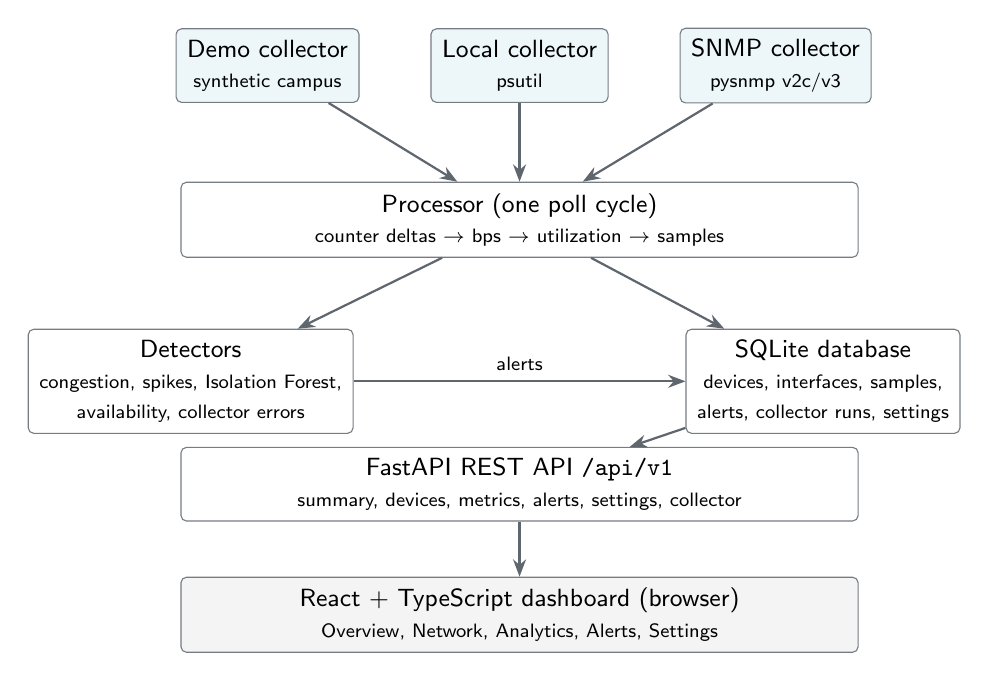
\begin{tikzpicture}[
  node distance=7mm and 9mm,
  box/.style={draw=ink!60, rounded corners=2pt, fill=white, align=center, font=\sffamily\small, minimum height=9mm, inner sep=4pt},
  src/.style={box, fill=accent!8},
  arr/.style={-{Stealth[length=2.2mm]}, draw=ink!70, thick}]
  \node[src] (demo) {Demo collector\\\scriptsize synthetic campus};
  \node[src, right=of demo] (local) {Local collector\\\scriptsize psutil};
  \node[src, right=of local] (snmp) {SNMP collector\\\scriptsize pysnmp v2c/v3};
  \node[box, below=10mm of local, minimum width=8.6cm] (proc) {Processor (one poll cycle)\\\scriptsize counter deltas $\rightarrow$ bps $\rightarrow$ utilization $\rightarrow$ samples};
  \node[box, below left=9mm and -22mm of proc] (det) {Detectors\\\scriptsize congestion, spikes, Isolation Forest,\\\scriptsize availability, collector errors};
  \node[box, below right=9mm and -22mm of proc] (db) {SQLite database\\\scriptsize devices, interfaces, samples,\\\scriptsize alerts, collector runs, settings};
  \node[box, below=24mm of proc, minimum width=8.6cm] (api) {FastAPI REST API \code{/api/v1}\\\scriptsize summary, devices, metrics, alerts, settings, collector};
  \node[box, below=7mm of api, minimum width=8.6cm, fill=ink!5] (ui) {React + TypeScript dashboard (browser)\\\scriptsize Overview, Network, Analytics, Alerts, Settings};
  \draw[arr] (demo) -- (proc); \draw[arr] (local) -- (proc); \draw[arr] (snmp) -- (proc);
  \draw[arr] (proc) -- (det); \draw[arr] (proc) -- (db); \draw[arr] (det) -- node[above, font=\scriptsize\sffamily]{alerts} (db);
  \draw[arr] (db) -- (api); \draw[arr] (api) -- (ui);
\end{tikzpicture}
\end{center}

\subsection{What happens in one poll cycle}

\begin{enumerate}
  \item The background poller wakes up (every 10\,s) and reads the active mode from the settings table.
  \item It builds the list of targets: demo devices, this computer, or the configured SNMP devices.
  \item The collector returns \emph{raw cumulative counters} plus reachability for each device. All three collectors return the
        same shape, so everything after this step is identical for demo and real data.
  \item The processor computes rates and utilization from the stored previous counters, updates each interface's latest values,
        and writes one sample row per interface (plus one per device for CPU and memory).
  \item The detectors run on each new sample and raise, update or resolve alerts.
  \item A \emph{collector run} row records what happened: devices polled, devices that failed and why, samples written.
  \item The browser refreshes on the same interval and reads everything through the REST API.
\end{enumerate}

\subsection{Database tables}

\begin{center}
\small
\begin{tabularx}{\linewidth}{@{}l Y@{}}
\toprule
\textbf{Table} & \textbf{Holds} \\
\midrule
\code{locations} & campus areas: name, subnet, VLAN, description \\
\code{devices} & name, IP, type, area, source mode, status (online/offline/unknown), last seen, CPU, memory, SNMP settings
                 (community and keys are write-only, never sent to the browser) \\
\code{interfaces} & per device: name, capacity and where it came from, oper status, last counters, latest rates and utilization \\
\code{metric\_samples} & one row per interface per poll: timestamp, bytes, bps, utilization, z-score, ML score, source mode \\
\code{alerts} & category, severity, status (active/resolved), acknowledged time, observed value, threshold, baseline, message,
                deduplication key, occurrence count \\
\code{collector\_runs} & every poll: mode, start/finish, success, error, per-device failures \\
\code{app\_settings} & the settings edited in the UI (mode, interval, thresholds, retention) \\
\bottomrule
\end{tabularx}
\end{center}

Every device, sample, alert and run is tagged with its \code{source\_mode}. Pages show only the active mode's data by default,
so synthetic and real data are never mixed. Old samples are purged after the retention period (7 days).

\subsection{The dashboard pages}

\begin{itemize}
  \item \textbf{Overview:} live throughput (in/out), devices up, active alerts, busiest link; the \emph{front panel}, which draws every
        interface as a switch port grouped by area (left LED shows link state and utilization colour, right LED blinks faster
        with more traffic); campus traffic chart; collector health; per-area comparison; recent alerts; devices needing attention.
  \item \textbf{Network \& Devices:} searchable, sortable tables of devices and interfaces (edit link capacity here); a view grouped
        by campus area; device detail with ports, traffic, CPU/memory and alerts.
  \item \textbf{Traffic Analytics:} time ranges 15\,min to 7\,days, area filter, trend chart, area comparison over time,
        most-used interfaces and devices, alert history by category.
  \item \textbf{Anomalies \& Alerts:} detector status and the \emph{Train now} button for the ML model, filters, the alert table,
        and a detail panel that explains why each alert fired, with an Acknowledge button.
  \item \textbf{Settings:} collection mode, poll interval, \emph{Poll now}, recent collector runs, thresholds, SNMP targets with a
        connection test, campus areas, demo data reset.
\end{itemize}

The header always shows the data source (\emph{Demo $\cdot$ synthetic} or \emph{Live}), when data was last updated, and a thin line
that fills until the next poll.

% ------------------------------------------------------------------ 5
\section{Installing and running}

\subsection{Requirements}
\begin{itemize}
  \item \textbf{Python 3.11 or newer} (tested with 3.13). Check with \code{python --version} (Windows: \code{py --version}).
  \item \textbf{Node.js 20.19+ or 22.12+} with npm. Check with \code{node --version}.
  \item No database server, Docker, internet services or passwords are needed for Demo mode.
\end{itemize}

\subsection{Install once}

\textbf{Windows (PowerShell)}, from the project folder:
\begin{lstlisting}
cd backend
py -3 -m venv .venv
.\.venv\Scripts\Activate.ps1
pip install -r requirements.txt
cd ..\frontend
npm install
\end{lstlisting}
If PowerShell refuses to run \code{Activate.ps1}, run this once and try again:
\begin{lstlisting}
Set-ExecutionPolicy -Scope CurrentUser RemoteSigned
\end{lstlisting}

\textbf{macOS / Linux:}
\begin{lstlisting}
cd backend
python3 -m venv .venv
source .venv/bin/activate
pip install -r requirements.txt
cd ../frontend
npm install
\end{lstlisting}

\subsection{Run (two terminals)}

\textbf{Terminal 1, backend} (port 8000):
\begin{lstlisting}
cd backend
.\.venv\Scripts\Activate.ps1        # macOS/Linux: source .venv/bin/activate
uvicorn app.main:app --host 127.0.0.1 --port 8000
\end{lstlisting}
The first start creates \file{backend/data/campus.db} and generates 24 hours of synthetic demo history (about 10 seconds; the log
prints \code{Demo seed: \{'seeded': True, ...\}}). Later starts reuse the data and never duplicate it.

\textbf{Terminal 2, frontend} (port 5173):
\begin{lstlisting}
cd frontend
npm run dev
\end{lstlisting}
Open \textbf{\url{http://127.0.0.1:5173}}. Quick checks: \url{http://127.0.0.1:8000/health} returns \code{"status":"ok"}, and
\url{http://127.0.0.1:8000/docs} shows the interactive API documentation (useful to show the professor).

\subsection{Tests and checks}
\begin{lstlisting}
cd backend   (venv active)
python -m pytest -q        # 23 tests, all should pass

cd frontend
npm run build              # type-check + production build
\end{lstlisting}
The tests cover the rate formula and its edge cases, congestion alerts (dedup, escalation, resolve, re-open), spike detection with
its explanation, unreachable devices, the API endpoints, settings validation, that SNMP secrets are never returned, and that an
unreachable SNMP target is reported without crashing.

\subsection{Demo data controls}
\begin{itemize}
  \item \textbf{Reset to a fresh demo:} Settings $\rightarrow$ Demo data $\rightarrow$ Reset \& reseed (asks for confirmation, about 10\,s).
  \item \textbf{Start completely fresh:} stop the backend, delete \file{backend/data/campus.db} (and the \code{-shm}/\code{-wal} files), start again.
  \item The demo is reproducible (fixed random seed 42). It follows the laptop's local time of day: the Student Area common-room
        Wi-Fi is busy (70 to 95\%) between 10:00 and 22:00, so a congestion alert is usually active during a daytime presentation.
\end{itemize}

\subsection{Optional: real SNMP without hardware}
The repository contains a simulated lab switch (\file{scripts/snmpsim/labswitch.snmprec}). In a \emph{separate} Python environment:
\begin{lstlisting}
python -m venv .simvenv            # then activate it
pip install snmpsim pysmi cryptography
snmpsim-command-responder --data-dir=scripts/snmpsim --agent-udpv4-endpoint=127.0.0.1:1161
\end{lstlisting}
In CampusWatch, add an SNMP target: address \code{127.0.0.1}, port \code{1161}, version v2c, community \code{labswitch}; switch to
SNMP mode. You will see real SNMP polling: one port at 100/20\,Mbps on a 1\,Gbps link, one at 80/10\,Mbps on a 100\,Mbps link
(which raises a congestion warning), and one port down.

% ------------------------------------------------------------------ 6
\section{Cisco Packet Tracer}

The companion PDF \file{docs/Packet\_Tracer\_Topology.pdf} builds the same campus in Packet Tracer: same device names, VLANs and
IPs, with step-by-step cabling, router and switch configurations (VLANs, trunks, router-on-a-stick, DHCP, SNMP) and the
verification commands to run live.

\begin{careful}
Packet Tracer is a simulator. Its devices exist only inside the program, so CampusWatch on your laptop cannot poll them.
That is exactly why the project has Demo mode. Show SNMP working \emph{inside} Packet Tracer with a PC's MIB Browser, then show the
dashboard in Demo mode and explain that SNMP mode does the same polling against real, reachable devices.
\end{careful}

% ------------------------------------------------------------------ 7
\section{Presentation demo script (about 10 minutes)}

\textbf{Before you start:} backend and frontend running, browser on the Overview page, Packet Tracer file open (optional).

\begin{tabularx}{\linewidth}{@{}p{0.4cm} >{\raggedright\arraybackslash}p{3.9cm} Y@{}}
\toprule
\textbf{\#} & \textbf{Show} & \textbf{Say} \\
\midrule
1 & Packet Tracer topology (optional) & ``This is the campus: four areas, each a VLAN and subnet, routed by one router.'' Run a ping between areas. \\
2 & Overview, header badge and banner & ``The source is always visible. Right now this is synthetic demo data, and the app says so on every page.'' \\
3 & Overview, front panel & ``Each square is a switch port, one per monitored interface, grouped by area. Green means link up, amber and red are the 70 and 90 percent thresholds, the right light blinks faster with more traffic.'' Point at a port to show its readout. \\
4 & Overview, wait 10\,s or press Refresh & ``Every 10 seconds we read the counters again. Rates come from the difference between readings.'' Numbers and chart update. \\
5 & Network \& Devices, then a device & ``Inventory with area, VLAN, status, last seen. The printer is offline, so its traffic is unavailable, not zero.'' Open \code{ACAD-LAB-PC-01}: no capacity configured, so no utilization. \\
6 & Traffic Analytics, range 24h & ``History: academic areas peak in lecture hours, the student area in the evening. Most-used links ranked.'' \\
7 & Alerts, filter Traffic anomaly, open one & ``The detector compares each sample with its rolling baseline. Here is the observed value, the baseline and the threshold, and the explanation.'' \\
8 & Alerts, a congestion alert, Acknowledge, press F5 & ``One alert per link, not one per poll; see the occurrence count. Acknowledged state is stored in the database, so it survives a refresh.'' \\
9 & Analytics, change ranges 15m to 7d & ``Every chart refetches for the range; the filters live in the URL.'' \\
10 & Settings & Show modes, thresholds and SNMP targets. Optionally add an unreachable target (\code{192.0.2.10}, community \code{public}), switch to SNMP, Poll now: the device shows offline with the timeout error and an alert appears. Switch back to Demo. \\
\bottomrule
\end{tabularx}

If something goes wrong during the demo: Settings $\rightarrow$ Demo data $\rightarrow$ Reset \& reseed, then refresh. If the banner says
``Backend unreachable'', the backend terminal was closed; start it again and the page recovers by itself.

% ------------------------------------------------------------------ 8
\section{Questions your professor may ask}

\qa{Why can't you show the speed from a single SNMP reading?}{Interface counters are cumulative totals since boot. Speed is a
change over time, so it needs two readings: $(\Delta\text{bytes} \times 8) / \Delta t$. The first poll of any interface
therefore shows no rate.}

\qa{What if the counter wraps or the device reboots?}{32-bit counters wrap at $2^{32}$ bytes; when the new value is smaller we add
$2^{32}$ once. 64-bit counters do not wrap in practice, so a smaller value there means the device rebooted, and we skip that
interval instead of reporting a huge or negative rate. Rates above 110\% of capacity are also discarded.}

\qa{Why do you prefer the HC (64-bit) counters?}{At 1\,Gbps a 32-bit byte counter wraps in about 34 seconds, so a delayed or
missed poll makes the rate ambiguous. 64-bit counters remove that problem.}

\qa{How is utilization calculated, and why the maximum of in and out?}{Busier direction divided by capacity. Ethernet is full
duplex, each direction has the full capacity, so the busier direction is what fills the link.}

\qa{What if you don't know the link speed?}{Then we show the rate but no utilization and no congestion alerts. Inventing a
percentage would be misleading. The capacity can be entered per interface in the Interfaces table.}

\qa{Which SNMP version do you use and why?}{Both v2c and v3 are supported. v3 is preferred because it authenticates (SHA) and
encrypts (AES). v2c sends the community string in clear text, so it is only acceptable read-only on an isolated lab network.
Credentials are stored locally and never sent to the browser.}

\qa{Which OIDs do you poll?}{IF-MIB: interface names, type, oper status, HC in/out octets (with 32-bit fallback), and speed;
sysDescr/sysUpTime for reachability; HOST-RESOURCES-MIB for CPU and memory where available. See Section 3.3.}

\qa{How do you avoid an alert every 10 seconds for the same problem?}{Each problem has a deduplication key (for example
\code{congestion:<interface>}). While it is active we update the same alert and count occurrences; it resolves automatically
when the condition clears, and if it comes back within the 10-minute cooldown the old alert is re-opened. Congestion also needs
two consecutive samples above the threshold.}

\qa{How does your anomaly detection work?}{A rolling baseline of the last 30 samples per interface. A sample is flagged when it
is at least 3 standard deviations above the mean \emph{and} at least 1.6 times the mean, on links above 1\,Mbps. The two
conditions together avoid false alarms on very steady or very noisy links. Spikes are kept out of the baseline.}

\qa{What does the Isolation Forest add, and can you trust it?}{It is an unsupervised model that scores how unusual a sample is
compared with the history, considering time of day and area. It is a secondary signal with low (info) severity. In Demo mode it
is trained on synthetic data, and the app says so; with real data it needs enough history before it means anything.}

\qa{Is the demo data fake?}{It is simulated, and labelled as such everywhere: a banner on every page, a badge on each device and
alert, and it is stored with \code{source\_mode = demo}. It goes through exactly the same rate calculation and detectors as real
data, which is why the demo is useful to show the logic. Local and SNMP modes measure real counters.}

\qa{Why not poll the Packet Tracer devices directly?}{Packet Tracer devices only exist inside the simulator and are not reachable
from the real laptop, and their SNMP support is limited. So the project shows SNMP inside Packet Tracer with the MIB Browser,
and uses Demo mode (same campus) for the dashboard. SNMP mode was tested against an SNMP agent simulator.}

\qa{Why SQLite? Would it scale?}{It needs no server, so the project runs on any laptop. Writes happen once per poll in one
transaction and the queries use indexes on (interface, time). For a large campus you would move samples to a time-series
database such as InfluxDB; the storage layer is isolated so that is a contained change.}

\qa{How long is data kept?}{7 days by default (configurable 1 to 90). Older samples, collector runs and resolved alerts are
purged hourly.}

\qa{Why a 10-second poll interval?}{A trade-off: short enough to see bursts and react quickly, long enough to keep load and
storage small. Any rate is an average over the interval, so bursts shorter than the interval are smoothed.}

\qa{How do VLANs relate to the dashboard?}{Each campus area is a VLAN with its own subnet. Devices are assigned to an area, and
traffic is summed per area for comparison. Inter-VLAN traffic is routed by the core router (router-on-a-stick in Packet Tracer).}

\qa{What is Local mode measuring?}{The real byte counters of this computer's network interfaces, read with \code{psutil} every
poll, through the same rate formula. It is the simplest way to show live, real measurement.}

\qa{How did you test it?}{23 automated backend tests (rate maths, detectors, alert lifecycle, API, validation, secrets, SNMP
failure). The frontend type-checks and builds. SNMP polling was verified end to end against the snmpsim agent simulator (rates within about 2\% and a congestion alert), and SNMPv3 credentials were verified with the right and a wrong key.}

\qa{What about security and privacy?}{It only collects counters, interface status and CPU/memory: no packet contents, no
browsing data, no user tracking. Services bind to localhost. SNMP secrets are write-only. It is meant for an authorised lab
network.}

\qa{What would you improve next?}{Time-of-day (seasonal) baselines, SNMP traps for instant notification, NetFlow/sFlow to see
\emph{who} uses the bandwidth, user accounts, and a time-series database for long history.}

% ------------------------------------------------------------------ 9
\section{Where the code is}

\begin{center}
\small
\begin{tabularx}{\linewidth}{@{}l Y@{}}
\toprule
\textbf{If asked about\ldots} & \textbf{Open} \\
\midrule
Rate formula and edge cases & \file{backend/app/services/rates.py} \\
One poll cycle (rates, samples, detectors) & \file{backend/app/services/poller.py} (\code{process()}) \\
Congestion detection & \file{backend/app/detection/congestion.py} \\
Spike (z-score) detection & \file{backend/app/detection/anomaly.py} \\
Isolation Forest & \file{backend/app/detection/ml.py} \\
Alert deduplication and cooldown & \file{backend/app/services/alerts.py} (\code{AlertBook}) \\
SNMP polling & \file{backend/app/collectors/snmp.py} \\
Local (psutil) polling & \file{backend/app/collectors/local.py} \\
Demo generator and demo campus & \file{backend/app/collectors/demo.py} \\
Database tables & \file{backend/app/models/\_\_init\_\_.py} \\
REST API & \file{backend/app/api/} (\code{metrics.py}, \code{inventory.py}, \code{alerts.py}, \code{system.py}) \\
Settings and defaults & \file{backend/app/core/config.py} \\
Tests & \file{backend/tests/} \\
Dashboard pages & \file{frontend/src/pages/} \\
Front panel (ports and LEDs) & \file{frontend/src/components/PortPanel.tsx} \\
Charts & \file{frontend/src/components/charts.tsx} \\
API client & \file{frontend/src/api/client.ts} \\
API types & \file{frontend/src/types/index.ts} \\
Visual design decisions & \file{DESIGN.md} \\
\bottomrule
\end{tabularx}
\end{center}

% ------------------------------------------------------------------ 10
\section{Design decisions and honest limitations}

\textbf{Decisions worth mentioning}
\begin{itemize}
  \item \textbf{Custom React dashboard instead of Streamlit}, as the specification required: full control over layout, live
        refresh and interaction.
  \item \textbf{Same pipeline for every mode:} collectors only return raw counters, so demo data exercises the real calculations
        and detectors.
  \item \textbf{Seeded history is generated by the real pipeline:} the 24 hours of demo history are produced by running the demo
        collector over past timestamps through the same processor, so the seeded alerts are genuine detector output.
  \item \textbf{Unavailable is not zero:} missing data shows ``n/a'' and gaps in charts.
\end{itemize}

\textbf{Limitations}
\begin{itemize}
  \item Area and campus totals add up interface rates; traffic that crosses several monitored interfaces (an access point and its
        switch uplink) is counted on each, so totals indicate load, not unique traffic.
  \item The baseline is short-term (last 30 samples), not seasonal; a sudden but legitimate surge (a lab session starting) can be flagged.
  \item SNMP was verified against a simulator, not physical campus switches. Packet Tracer devices cannot be polled.
  \item Wi-Fi utilization is approximated (wireless airtime is shared, not full duplex).
  \item Single-user local tool: no login, no email notifications (optional in the specification).
\end{itemize}

% ------------------------------------------------------------------ 11
\section{Troubleshooting}

\begin{center}
\small
\begin{tabularx}{\linewidth}{@{}>{\raggedright\arraybackslash}p{5.2cm} Y@{}}
\toprule
\textbf{Problem} & \textbf{Fix} \\
\midrule
``Backend unreachable'' in the browser & Start the backend (Terminal 1). The page reconnects automatically. \\
\code{Address already in use} & Another program uses port 8000 or 5173. Close it, or run the backend on another port and start the
frontend with \code{VITE\_API\_PROXY=http://127.0.0.1:8010} \code{npm run dev}. \\
\code{Activate.ps1 cannot be loaded} & \code{Set-ExecutionPolicy -Scope CurrentUser RemoteSigned}, or run
\code{.\textbackslash.venv\textbackslash Scripts\textbackslash python -m uvicorn app.main:app --port 8000}. \\
Vite says Node is too old & Install Node.js 22 LTS. \\
Charts empty after switching to Local or SNMP & Rates need two polls and history builds over time; Demo mode has 24 hours ready. \\
Utilization shows n/a & Link capacity unknown: set it with the pencil icon in Network $\rightarrow$ Interfaces. \\
SNMP target offline with a timeout & Wrong IP, port, community or credentials, a firewall, or SNMP disabled. Use the Test button. \\
SNMPv3 ``Ciphering services not available'' & \code{pip install -r requirements.txt} (needs the \code{cryptography} package). \\
ML model ``Not trained'' & Needs 300 samples of the active mode; press Train now on the Alerts page. \\
Anything odd & Stop the backend, delete \file{backend/data/campus.db*}, start again. \\
\bottomrule
\end{tabularx}
\end{center}

% ------------------------------------------------------------------ 12
\section{Glossary}

\begin{description}[style=nextline, leftmargin=1.2cm, font=\sffamily\bfseries]
  \item[bps, Mbps, Gbps] bits per second; $10^6$ and $10^9$ bits per second. Link speeds use bits, counters count bytes.
  \item[Counter (octet counter)] a running total of bytes through an interface since it started.
  \item[Utilization] traffic as a percentage of link capacity.
  \item[SNMP] Simple Network Management Protocol: a manager reads values from agents on network devices (UDP 161).
  \item[MIB, OID] the tree of values a device exposes, and the numeric address of one value in it.
  \item[IF-MIB] the standard MIB module for network interfaces (names, status, counters, speed).
  \item[Community string] the shared password of SNMP v1/v2c, sent unencrypted.
  \item[VLAN] a virtual LAN: a separate broadcast domain on shared switches, identified by a number (10, 20, 30, 100).
  \item[Trunk] a link that carries several VLANs, tagging frames with IEEE 802.1Q.
  \item[Router-on-a-stick] inter-VLAN routing with one router port split into sub-interfaces, one per VLAN.
  \item[Rolling baseline] the average and spread of the most recent samples, used as ``normal''.
  \item[z-score] how many standard deviations a value is from the mean.
  \item[Isolation Forest] an unsupervised algorithm that scores how easily a point can be separated from the rest; unusual points
        separate quickly.
  \item[Deduplication / cooldown] keeping one alert per ongoing problem / re-opening it instead of creating a new one if it returns soon.
  \item[Source mode] where data came from: demo (synthetic), local (this computer), snmp (network devices).
\end{description}

\end{document}
